\documentclass[12pt, openany, oneside]{book}

\usepackage{listings}
\usepackage[dvipsnames]{xcolor}
\usepackage{ctex}
\usepackage{fontspec}
\usepackage{setspace}
\usepackage{tikz}
\usepackage{anyfontsize}
\usepackage{sectsty}
\usepackage{titlesec}
\usepackage{float}
\usepackage[hidelinks]{hyperref}
\usepackage[a4paper]{geometry}
\usepackage{url}
\usepackage{amssymb}
\usepackage{fontawesome5}
\usepackage[most]{tcolorbox}
\usepackage{stackengine}
\usepackage{multirow}
\usepackage[T1]{fontenc}
\usepackage{diagbox}
\usepackage{longtable}
\usepackage{newtxtt}
\usepackage{pgf-umlcd}
\usepackage{bbding}
\usepackage[edges]{forest}

\usetikzlibrary{calc,trees,positioning,arrows,fit,shapes}
\usetikzlibrary{shapes.multipart,chains}
\usetikzlibrary{shadows}

\makeatletter
\newcommand{\verbatimfont}[1]{\renewcommand{\verbatim@font}{\ttfamily#1}}
\makeatother

\tikzstyle{startend} = [rectangle, rounded corners, minimum width=3cm, minimum height=1cm, text centered, draw=black, fill=red!30]
\tikzstyle{io}        = [trapezium, trapezium left angle=70, trapezium right angle=110, minimum width=3cm, inner xsep = -15pt, minimum height=1cm, text centered, draw=black, fill=blue!30]
\tikzstyle{process}   = [rectangle, minimum width=3cm, minimum height=1cm, inner ysep=0, text centered, draw=black, fill=orange!30]
\tikzstyle{decision}  = [diamond,shape aspect=2.5, minimum width=3cm, minimum height=1cm, inner xsep=0,text centered, draw=black, fill=green!30]
\tikzstyle{arrow}     = [thick,->,>=stealth]

\def\rlwd{.5pt} \def\rlht{2.2ex} \def\rldp{.5ex}
\def\mydiv#1{~
  \rule[-\rldp]{\rlwd}{\rlht}
  \setbox0=\hbox{~#1}
  \stackunder[\dimexpr\rldp-\rlwd]{~#1}{\rule{\wd0}{\rlwd}}%
}

\definecolor{mycolor}{RGB}{0,128,128}
\newtcbox{\mybox} {
    on line,
    colback=mycolor,
    fontupper=\bfseries\color{white},
    boxrule=0pt,
    arc=5pt, 
    boxsep=0pt, 
    left=2pt, 
    right=2pt, 
    top=5pt, 
    bottom=5pt
}

\setstretch{1.5}
\setlength{\parindent}{0cm}

\geometry{a4paper,top=2.5cm,bottom=2.5cm}

\titleformat{\chapter}{\Huge\Huge\bfseries}{\chaptertitlename\ \thechapter{\ }}{0pt}{\Huge}{}
\titlespacing{\chapter}{0pt}{0pt}{12pt}

\definecolor{dkgreen}{rgb}{0,0.4,0}
\definecolor{gray}{rgb}{0.5,0.5,0.5}
\definecolor{mauve}{rgb}{0.58,0,0.82}
\definecolor{LightGray}{gray}{0.9}

\lstset{
    basicstyle=\linespread{1.3} \fontspec{Consolas},    %  the size of the fonts that are used for the code
	basewidth=0.5em,
    numbers=left,            % where to put the line-numbers
    numberstyle=\color{black},  % the style that is used for the line-numbers
    numbersep=10pt,                  % how far the line-numbers are from the code
    backgroundcolor=\color{white},
    showspaces=false,
    showstringspaces=false,
    showtabs=false,
    frame=single,                   % adds a frame around the code
    rulecolor=\color{black},        % if not set, the frame-color may be changed on line-breaks within not-black text (e.g. commens (green here))
    tabsize=4,                      % sets default tabsize to 2 spaces
    captionpos=t,                   % sets the caption-position to bottom
    breaklines=false,                % sets automatic line breaking
    breakatwhitespace=true,        % sets if automatic breaks should only happen at whitespace
    title=\lstname,                   % show the filename of files included with \lstinputlisting;
    % also try caption instead of title
    numberstyle=\color{black},		% line number color
    keywordstyle=\color{blue},          % keyword style
    commentstyle=\color{dkgreen},       % comment style
    stringstyle=\color{mauve},         % string literal style
    escapeinside={\%*}{*)},            % if you want to add LaTeX within your code
    morekeywords={*,...}               % if you want to add more keywords to the set
}

\begin{document}

\thispagestyle{empty}

\begin{tikzpicture}[overlay,remember picture]
	\fill[
		black!2]
	(current page.south west) rectangle (current page.north east);

	\shade[
		left color=Dandelion,
		right color=Dandelion!40,
		transform canvas ={rotate around ={45:($(current page.north west)+(0,-6)$)}}]
	($(current page.north west)+(0,-6)$) rectangle ++(9,1.5);

	\shade[
		left color=lightgray,
		right color=lightgray!50,
		rounded corners=0.75cm,
		transform canvas ={rotate around ={45:($(current page.north west)+(.5,-10)$)}}]
	($(current page.north west)+(0.5,-10)$) rectangle ++(15,1.5);

	\shade[
		left color=lightgray,
		rounded corners=0.3cm,
		transform canvas ={rotate around ={45:($(current page.north west)+(.5,-10)$)}}] ($(current page.north west)+(1.5,-9.55)$) rectangle ++(7,.6);

	\shade[
		left color=orange!80,
		right color=orange!60,
		rounded corners=0.4cm,
		transform canvas ={rotate around ={45:($(current page.north)+(-1.5,-3)$)}}]
	($(current page.north)+(-1.5,-3)$) rectangle ++(9,0.8);

	\shade[
		left color=red!80,
		right color=red!80,
		rounded corners=0.9cm,
		transform canvas ={rotate around ={45:($(current page.north)+(-3,-8)$)}}] ($(current page.north)+(-3,-8)$) rectangle ++(15,1.8);

	\shade[
		left color=orange,
		right color=Dandelion,
		rounded corners=0.9cm,
		transform canvas ={rotate around ={45:($(current page.north west)+(4,-15.5)$)}}]
	($(current page.north west)+(4,-15.5)$) rectangle ++(30,1.8);

	\shade[
		left color=RoyalBlue,
		right color=Emerald,
		rounded corners=0.75cm,
		transform canvas ={rotate around ={45:($(current page.north west)+(13,-10)$)}}]
	($(current page.north west)+(13,-10)$) rectangle ++(15,1.5);

	\shade[
		left color=lightgray,
		rounded corners=0.3cm,
		transform canvas ={rotate around ={45:($(current page.north west)+(18,-8)$)}}]
	($(current page.north west)+(18,-8)$) rectangle ++(15,0.6);

	\shade[
		left color=lightgray,
		rounded corners=0.4cm,
		transform canvas ={rotate around ={45:($(current page.north west)+(19,-5.65)$)}}]
	($(current page.north west)+(19,-5.65)$) rectangle ++(15,0.8);

	\shade[
		left color=OrangeRed,
		right color=red!80,
		rounded corners=0.6cm,
		transform canvas ={rotate around ={45:($(current page.north west)+(20,-9)$)}}]
	($(current page.north west)+(20,-9)$) rectangle ++(14,1.2);

	% Title
	\node[align=center] at ($(current page.center)+(0,-5)$)
	{
	{\fontsize{72}{72} \selectfont {{C}}}\\[2cm]
	{\fontsize{20}{19.2} \selectfont \textcolor{orange}{ \bf 极夜酱}}\\[4pt]
	};
\end{tikzpicture}

\newpage

\pagestyle{plain}
\setcounter{page}{1}
\setcounter{tocdepth}{1}
\tableofcontents

\newpage

\setcounter{page}{1}

% \chapter{C简介}

\section{编程简介}

\subsection{编程简介}

程序(program)是为了让计算机执行某些操作或者解决问题而编写的一系列有序指令的集合。由于计算机只能够识别二进制数字0和1,因此需要使用特殊的编程语言来描述如何解决问题过程和方法。\\

算法(algorithm)是可完成特定任务的一系列步骤,算法的计算过程定义明确,通过一些值作为输入并产生一些值作为输出。\\

流程图(flow chart)是算法的一种图形化表示方式,使用一组预定义的符号来说明如何执行特定任务。

\begin{itemize}
	\item 圆角矩形:开始和结束
	\item 矩形:数据处理
	\item 平行四边形:输入/输出
	\item 菱形:分支判断条件
	\item 流程线:步骤
\end{itemize}

\begin{figure}
	\centering
	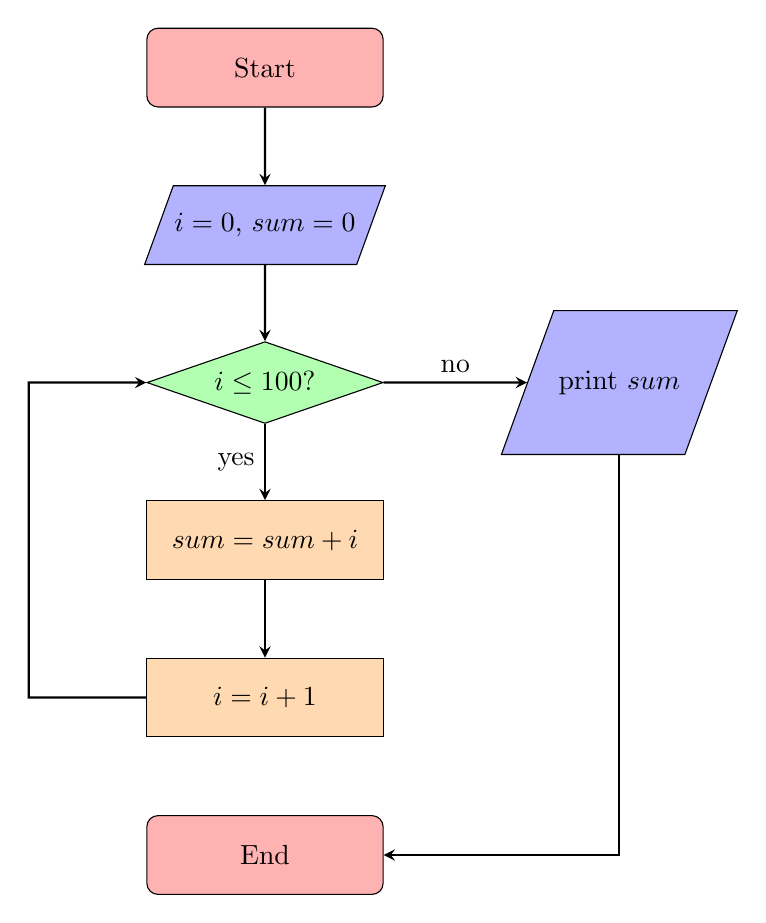
\begin{tikzpicture}[node distance=2cm]
		\node (start) [startend] {Start};
		\node (init)   [io, below of=start] {$ i = 0 $, $ sum = 0 $};
		\node (decision)  [decision, below of=init] {$ i \le 100 $?};
		\node (accumulation) [process, below of=decision] {$ sum = sum + i $};
		\node (update) [process, below of=accumulation] {$ i = i + 1 $};
		\node (output) [io, right of=decision, xshift=2.5cm] {print $ sum $};
		\node (end) [startend, below of=update] {End};

		\draw [arrow] (start) -- (init);
		\draw [arrow] (init) -- (decision);
		\draw [arrow] (decision) -- node[anchor=east] {yes } (accumulation);
		\draw [arrow] (accumulation) -- (update);
		\draw [arrow] (update) -- (-3,-8) -- (-3,-4) -- (decision);
		\draw [arrow] (decision) -- node[anchor=south] {no} (output);
		\draw [arrow] (output) |- (end);
	\end{tikzpicture}
	\caption{计算$ \sum_{i=1}^{100} i $的流程图}
\end{figure}

\vspace{0.5cm}

\subsection{编程语言(Programming Language)}

编程语言主要分为面向机器、面向过程和面向对象三类。C是面向过程的语言,常用于操作系统、嵌入式系统、驱动程序、图形引擎、图像处理、声音效果等。\\

C是一个结构化的编程语言,因此它层次清晰便于按模块化方式组织程序,易于调试和维护。然而结构化的缺点也很明显,比如程序的可重用性差。

\begin{figure}[H]
	\centering
	
\includegraphics[scale=0.9]{img/C1/1-1/1.png}
	\caption{常见编程语言}
\end{figure}

\newpage

\section{Hello World!}

\subsection{Hello World!}

\mybox{Hello World!}

\begin{lstlisting}[language=C]
#include <stdio.h>

int main()
{
	printf("Hello World!\n");
	return 0;
}
\end{lstlisting}

\begin{tcolorbox}
	\mybox{运行结果}
	\begin{verbatim}
Hello World!
	\end{verbatim}
\end{tcolorbox}

第一行语句为预处理指令,预处理指令以【\#】开头,\#include表示程序需要使用头文件stdio.h中的函数,stdio.h文件中包含了有关输入输出语句的函数。\\

main()是C程序的入口,在程序的主体部分,printf()的功能是在屏幕上输出"Hello World"这个字符串,$ \backslash $n表示换行符。\\

C中【;】表示语句结束,注意不要使用中文的分号。一条语句可以跨越多行,并且用分号通知编译器该语句结束。\\

编译器(compiler)将程序编译成计算机能够识别的二进制文件,最终能够被计算机执行。

\newpage

\section{Error or Warning?}

\subsection{Error / Warning}

在编写程序的过程中,错误是不可避免的,错误主要能够分为以下三种类别:

\begin{enumerate}
	\item 语法错误(syntax error):程序的语法不合符编程语言的要求,编译器会反馈报错信息。

	\item 逻辑错误(logical error):人类在编程过程中的逻辑错误,无法被编译器所检测。

	\item 运行时错误(runtime error)例如除以0、数组越界、指针越界、使用已经释放的空间、栈溢出等情况,可以被编译器发现。
\end{enumerate}

\newpage

\section{注释}

\subsection{注释(Comment)}

在编程中加入注释可以增加程序的可读性和可维护性,编译器不会对注释的部分进行编译。\\

C中注释分为两类:

\begin{enumerate}
	\item 单行注释:将一行内【//】之后的内容视为注释。
	\item 多行注释:以【/*】开始,【*/】结束,中间的内容视为注释。
\end{enumerate}

\mybox{注释}

\begin{lstlisting}[language=C]
/*
    这个程序在屏幕上是输出Hello World
*/
#include <stdio.h>              // 头文件

int main()
{
    printf("Hello World!\n");   // 输出
    return 0;
}
\end{lstlisting}

\begin{tcolorbox}
	\mybox{运行结果}
	\begin{verbatim}
Hello World!
	\end{verbatim}
\end{tcolorbox}

\newpage

\section{不同语言的Hello World}

\subsection{编程语言对比}

\mybox{C++}

\begin{lstlisting}[language=C++]
#include <iostream>
using namespace std;

int main() {
	cout << "Hello World" << endl;
	return 0;
}
\end{lstlisting}

\vspace{0.5cm}

\mybox{Java}

\begin{lstlisting}[language=Java]
public class HelloWorld {
    public static void main(String[] args) {
        System.out.println("Hello World");
    }
}
\end{lstlisting}

\vspace{0.5cm}

\mybox{Python}

\begin{lstlisting}[language=Python]
print("Hello World")
\end{lstlisting}

\newpage
% \chapter{分支}

\section{逻辑运算符}

\subsection{关系运算符}

编程中经常需要使用关系运算符来比较两个数据的大小,比较的结果是一个布尔值(boolean),即True(非0)或False(0)。\\

在编程中需要注意,一个等号=表示赋值运算,而两个等号==表示比较运算。\\

\begin{table}[H]
	\centering
	\setlength{\tabcolsep}{5mm}{
		\begin{tabular}{|c|c|}
			\hline
			\textbf{数学符号} & \textbf{关系运算符} \\
			\hline
			$ < $             & <                   \\
			\hline
			$ > $             & >                   \\
			\hline
			$ \le $           & <=                  \\
			\hline
			$ \ge $           & >=                  \\
			\hline
			$ = $             & ==                  \\
			\hline
			$ \ne $           & !=                  \\
			\hline
		\end{tabular}
	}
\end{table}

\vspace{0.5cm}

\subsection{逻辑运算符}

逻辑运算符用于连接多个关系表达式,其结果也是一个布尔值。\\

\begin{enumerate}
	\item 逻辑与\&\&:当多个条件全部为True,结果为True。\\
	      \begin{table}[H]
		      \centering
		      \setlength{\tabcolsep}{5mm}{
			      \begin{tabular}{|c|c|c|}
				      \hline
				      \textbf{条件1} & \textbf{条件2} & \textbf{条件1 \&\& 条件2} \\
				      \hline
				      T              & T              & T                         \\
				      \hline
				      T              & F              & F                         \\
				      \hline
				      F              & T              & F                         \\
				      \hline
				      F              & F              & F                         \\
				      \hline
			      \end{tabular}
		      }
	      \end{table}

	\item 逻辑或||:多个条件至少有一个为True时,结果为True。\\
	      \begin{table}[H]
		      \centering
		      \setlength{\tabcolsep}{5mm}{
			      \begin{tabular}{|c|c|c|}
				      \hline
				      \textbf{条件1} & \textbf{条件2} & \textbf{条件1 || 条件2} \\
				      \hline
				      T              & T              & T                       \\
				      \hline
				      T              & F              & T                       \\
				      \hline
				      F              & T              & T                       \\
				      \hline
				      F              & F              & F                       \\
				      \hline
			      \end{tabular}
		      }
	      \end{table}

	\item 逻辑非!:条件为True时,结果为False;条件为False时,结果为True。\\
	      \begin{table}[H]
		      \centering
		      \setlength{\tabcolsep}{5mm}{
			      \begin{tabular}{|c|c|}
				      \hline
				      \textbf{条件} & \textbf{!条件} \\
				      \hline
				      T             & F              \\
				      \hline
				      F             & T              \\
				      \hline
			      \end{tabular}
		      }
	      \end{table}
\end{enumerate}

\newpage

\section{if}

\subsection{if}

if语句用于判断一个条件是否成立,如果成立则进入语句块,否则不执行。\\

\mybox{年龄}

\begin{lstlisting}[language=C]
#include <stdio.h>

int main()
{
	int age;
	printf("Enter your age: ");
	scanf("%d", &age);
	if(age > 0 && age < 18)
	{
		printf("Minor\n");
	}
	return 0;
}
\end{lstlisting}

\begin{tcolorbox}
	\mybox{运行结果}
	\begin{verbatim}
Enter your age: 17
Minor
\end{verbatim}
\end{tcolorbox}

\vspace{0.5cm}

\subsection{if-else}

if-else的结构与if类似,只是在if语句块中的条件不成立时,执行else语句块中的语句。\\

\mybox{闰年}

\begin{lstlisting}[language=C]
#include <stdio.h>

int main()
{
	int year;
	printf("Enter a year: ");
	scanf("%d", &year);

	/*
	 * A year is a leap year if it is
	 * 1. exactly divisible by 4, and not divisible by 100;
	 * 2. or is exactly divisible by 400
	 */
	if((year % 4 == 0 && year % 100 != 0) || year % 400 == 0)
	{
		printf("Leap year\n");
	}
	else
	{
		printf("Common year\n");
	}

	return 0;
}
\end{lstlisting}

\begin{tcolorbox}
	\mybox{运行结果}
	\begin{verbatim}
Enter a year: 2020
Leap year
\end{verbatim}
\end{tcolorbox}

\vspace{0.5cm}

\subsection{if-else if-else}

当需要对更多的条件进行判断时,可以使用if-else if-else语句。\\

\mybox{字符}

\begin{lstlisting}[language=C]
#include <stdio.h>

int main()
{
	printf("Enter a character: ");
	char c = getchar();

	if(c >= 'a' && c <= 'z')
	{
		printf("Lowercase\n");
	}
	else if(c >= 'A' && c <= 'Z')
	{
		printf("Uppercase\n");
	}
	else if(c >= '0' && c <= '9')
	{
		printf("Digit\n");
	}
	else
	{
		printf("Special character\n");
	}
	
	return 0;
}
\end{lstlisting}

\begin{tcolorbox}
	\mybox{运行结果}
	\begin{verbatim}
Enter a character: T
Uppercase
\end{verbatim}
\end{tcolorbox}

\newpage

\section{switch}

\subsection{switch}

switch结构用于根据一个整数值,选择对应的case执行。需要注意的是,当对应的case中的代码被执行完后,并不会像if语句一样跳出switch结构,而是会继续向后执行,直到遇到break。\\

\mybox{计算器}

\begin{lstlisting}[language=C]
#include <stdio.h>

int main() {
	int num1, num2;
	char operator;

	printf("Enter an expression: ");
	scanf("%d %c %d", &num1, &operator, & num2);

	switch (operator)
	{
	case '+':
		printf("%d + %d = %d\n", num1, num2, num1 + num2);
		break;
	case '-':
		printf("%d - %d = %d\n", num1, num2, num1 - num2);
		break;
	case '*':
		printf("%d * %d = %d\n", num1, num2, num1 * num2);
		break;
	case '/':
		printf("%d / %d = %d\n", num1, num2, num1 / num2);
		break;
	default:
		printf("Error! Operator is not supported\n");
		break;
	}

	return 0;
}
\end{lstlisting}

\begin{tcolorbox}
	\mybox{运行结果}
	\begin{verbatim}
Enter an expression: 5 * 8
5 * 8 = 40
\end{verbatim}
\end{tcolorbox}

\newpage
% \chapter{循环}

\section{while}

\subsection{while}

while循环会对条件进行判断,如果条件成立,就会执行循环体,然后再次判断条件,直到条件不成立。\\

while循环的次数由循环变量的变化决定,因此while循环一般都包括对循环变量的初值、判断和更新。

\begin{lstlisting}[language=C]
int i = 1;          // initial value
while(i <= 5)       // condition
{
    printf("In loop: i = %d\n", i);
    i++;            // update
}
printf("After loop: i = %d\n", i);
\end{lstlisting}

while循环的特点是先判断、再执行,因此循环体有可能会执行一次或多次,也有可能一次也不会执行。\\

\mybox{平均身高}

\begin{lstlisting}[language=C]
#include <stdio.h>
#define NUM_PEOPLE 5

int main()
{
    double height;
    double total = 0;

    int i = 1;
    while (i <= NUM_PEOPLE)
    {
        printf("Enter person %d's height: ", i);
        scanf("%lf", &height);
        total += height;
        i++;
    }

    double average = total / NUM_PEOPLE;
    printf("Average height: %.2f\n", average);
    return 0;
}
\end{lstlisting}

\begin{tcolorbox}
    \mybox{运行结果}
    \begin{verbatim}
Enter person 1's height: 160.8
Enter person 2's height: 175.2
Enter person 3's height: 171.2
Enter person 4's height: 181.3
Enter person 5's height: 164
Average height: 170.50
\end{verbatim}
\end{tcolorbox}

\vspace{0.5cm}

\mybox{统计元音、辅音数量}

\begin{lstlisting}[language=C]
#include <stdio.h>

int main()
{
    char c;
    int vowel = 0;
    int consonant = 0;

    printf("Enter an English sentence: ");

    while ((c = getchar()) != '\n')
    {
        if (c == 'a' || c == 'A' ||
            c == 'e' || c == 'E' || 
            c == 'i' || c == 'I' || 
            c == 'o' || c == 'O' || 
            c == 'u' || c == 'U')
        {
            vowel++;
        }
        else if ((c >= 'a' && c <= 'z') || (c >= 'A' && c <= 'Z'))
        {
            consonant++;
        }
    }

    printf("Vowel = %d\n", vowel);
    printf("Consonant = %d\n", consonant);
    return 0;
}
\end{lstlisting}

\begin{tcolorbox}
    \mybox{运行结果}
    \begin{verbatim}
Enter an English sentence: Hello World!
Vowel = 3
Consonant = 7
\end{verbatim}
\end{tcolorbox}

\vspace{0.5cm}

\subsection{do-while}

do-while循环是先执行一轮循环体内的代码后,再检查循环的条件是否成立。如果成立,则继续下一轮循环;否则循环结束。\\

do-while循环是先执行、再判断,因此它至少会执行一轮循环。do-while一般应用在一些可能会需要重复,但必定会发生一次的情景下。例如登录账户,用户输入账户和密码后,检查是否正确,如果正确,那么就成功登录;否则继续循环让用户重新输入。\\

需要注意,do-while循环的最后有一个分号。

\begin{lstlisting}[language=C]
do {
    // code
} while(condition);
\end{lstlisting}

\vspace{0.5cm}

\mybox{整数位数}

\begin{lstlisting}[language=C]
#include <stdio.h>

int main()
{
    int num;
    int n = 0;

    printf("Enter an integer: ");
    scanf("%d", &num);

    do
    {
        num /= 10;
        n++;
    } while(num != 0);

    printf("Digits: %d\n", n);
    return 0;
}
\end{lstlisting}

\begin{tcolorbox}
    \mybox{运行结果}
    \begin{verbatim}
Enter an integer: 123
Digits: 3
\end{verbatim}
\end{tcolorbox}

\vspace{0.5cm}

\mybox{猜数字}

\begin{lstlisting}[language=C]
#include <stdio.h>
#include <stdlib.h>
#include <time.h>

int main()
{
    srand(time(NULL));          // set random seed

    // generate random number between 1 and 100
    int answer = rand() % 100 + 1;
    int num = 0;
    int cnt = 0;

    do
    {
        printf("Guess a number: ");
        scanf("%d", &num);
        cnt++;
        
        if(num > answer)
        {
            printf("Too high\n");
        }
        else if(num < answer)
        {
            printf("Too low\n");
        }
    } while(num != answer);
    
    printf("Correct! You guessed %d times.\n", cnt);
    return 0;
}
\end{lstlisting}

\begin{tcolorbox}
    \mybox{运行结果}
    \begin{verbatim}
Guess a number: 50
Too high
Guess a number: 25
Too low
Guess a number: 37
Too low
Guess a number: 43
Too high
Guess a number: 40
Too high
Guess a number: 38
Too low
Guess a number: 39
Correct! You guessed 7 times.
\end{verbatim}
\end{tcolorbox}

\newpage

\section{for}

\subsection{for}

while循环将循环变量的初值、条件和更新写在了三个地方,但是这样不容易明显地看出循环变量的变化。\\

for循环将循环变量的初值、条件和更新写在了一行内,中间用分号隔开。对于指定次数的循环一般更多地会采用for循环,而对于不确定次数的一般会采用while循环。

\begin{lstlisting}[language=C]
for(int i = 0; i < 5; i++)
{
    printf("i = %d\n", i);
}
\end{lstlisting}

\vspace{0.5cm}

\mybox{累加}

\begin{lstlisting}[language=C]
#include <stdio.h>

int main()
{
    int sum = 0;
    for(int i = 1; i <= 100; i++)
    {
        sum += i;
    }
    printf("Sum = %d\n", sum);
    return 0;
}
\end{lstlisting}

\begin{tcolorbox}
    \mybox{运行结果}
    \begin{verbatim}
Sum = 5050
\end{verbatim}
\end{tcolorbox}

\vspace{0.5cm}

\mybox{斐波那契数列}

\begin{figure}[H]
    \centering
    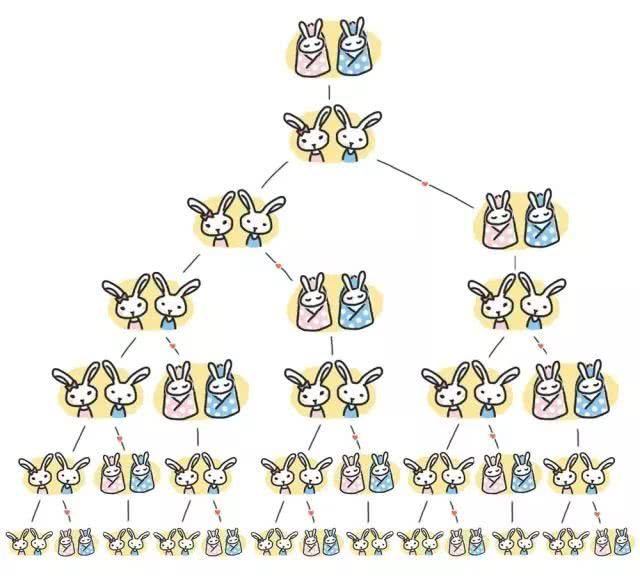
\includegraphics[scale=0.5]{img/Chapter3/3-2/1.png}
\end{figure}

\begin{lstlisting}[language=C]
#include <stdio.h>

int main()
{
    int n;
    printf("Enter the number of terms: ");
    scanf("%d", &n);

    if(n == 1)
    {
        printf("1\n");
    }
    else if(n == 2)
    {
        printf("1, 1\n");
    }
    else
    {
        int num1, num2, val;
        num1 = 1;
        num2 = 1;
        printf("1, 1");

        for(int i = 3; i <= n; i++)
        {
            val = num1 + num2;
            printf(", %d", val);
            num1 = num2;
            num2 = val;
        }
        printf("\n");
    }
    
    return 0;
}
\end{lstlisting}

\begin{tcolorbox}
    \mybox{运行结果}
    \begin{verbatim}
Enter the number of terms: 10
1, 1, 2, 3, 5, 8, 13, 21, 34, 55
\end{verbatim}
\end{tcolorbox}

\vspace{0.5cm}

\subsection{嵌套循环}

循环也可以嵌套使用,外层循环每执行一次,内层循环就会执行多次。

\begin{lstlisting}[language=C]
for(int i = 0; i < 2; i++)
{
    for(int j = 0; j < 3; j++)
    {
        printf("i = %d, j = %d\n", i, j);
    }
}
\end{lstlisting}

\begin{tcolorbox}
    \mybox{运行结果}
    \begin{verbatim}
i = 0, j = 0
i = 0, j = 1
i = 0, j = 2
i = 1, j = 0
i = 1, j = 1
i = 1, j = 2
\end{verbatim}
\end{tcolorbox}

\vspace{0.5cm}

\mybox{九九乘法表}\\

\begin{table}[H]
    \centering
    \setlength{\tabcolsep}{1.5mm}{
        \begin{tabular}{|c|c|c|c|c|c|c|c|c|}
            \hline
            1*1=1 & 1*2=2  & 1*3=3  & 1*4=4  & 1*5=5  & 1*6=6  & 1*7=7  & 1*8=8  & 1*9=9  \\
            \hline
            2*1=2 & 2*2=4  & 2*3=6  & 2*4=8  & 2*5=10 & 2*6=12 & 2*7=14 & 2*8=16 & 2*9=18 \\
            \hline
            3*1=3 & 3*2=6  & 3*3=9  & 3*4=12 & 3*5=15 & 3*6=18 & 3*7=21 & 3*8=24 & 3*9=27 \\
            \hline
            4*1=4 & 4*2=8  & 4*3=12 & 4*4=16 & 4*5=20 & 4*6=24 & 4*7=28 & 4*8=32 & 4*9=36 \\
            \hline
            5*1=5 & 5*2=10 & 5*3=15 & 5*4=20 & 5*5=25 & 5*6=30 & 5*7=35 & 5*8=40 & 5*9=45 \\
            \hline
            6*1=6 & 6*2=12 & 6*3=18 & 6*4=24 & 6*5=30 & 6*6=36 & 6*7=42 & 6*8=48 & 6*9=54 \\
            \hline
            7*1=7 & 7*2=14 & 7*3=21 & 7*4=28 & 7*5=35 & 7*6=42 & 7*7=49 & 7*8=56 & 7*9=63 \\
            \hline
            8*1=8 & 8*2=16 & 8*3=24 & 8*4=32 & 8*5=40 & 8*6=48 & 8*7=56 & 8*8=64 & 8*9=72 \\
            \hline
            9*1=9 & 9*2=18 & 9*3=27 & 9*4=36 & 9*5=45 & 9*6=54 & 9*7=63 & 9*8=72 & 9*9=81 \\
            \hline
        \end{tabular}
    }
\end{table}

\begin{lstlisting}[language=C]
#include <stdio.h>

int main()
{
    for(int i = 1; i <= 9; i++)
    {
        for(int j = 1; j <= 9; j++)
        {
            printf("%d*%d=%d\t", i, j, i*j);
        }
        printf("\n");
    }
    return 0;
}
\end{lstlisting}

\vspace{0.5cm}

\mybox{打印图案}

\begin{lstlisting}
*
**
***
****
*****
\end{lstlisting}

\begin{lstlisting}[language=C]
#include <stdio.h>

int main()
{
    for(int i = 1; i <= 5; i++)
    {
        for(int j = 1; j <= i; j++)
        {
            printf("*");
        }
        printf("\n");
    }
    return 0;
}
\end{lstlisting}

\newpage

\section{break or continue?}

\subsection{break}

break可用于跳出当前的switch或循环结构。在一些情况下,在循环的中途已经完成了某个目标,没有必要再进行剩余的循环,这时就可以使用break跳出循环。\\

例如在判断一个数$ n $是否为素数时,利用循环逐个判断$ 2 \sim n - 1 $之间的数是否能整除$ n $。只要发现其中有一个数能整除$ n $,就证明$ n $不是素数,可以跳出循环,不必再进行剩余的检查。\\

\mybox{素数}

\begin{lstlisting}[language=C]
#include <stdio.h>
#include <stdbool.h>
#include <math.h>

int main()
{
    int n;
    printf("Enter an integer: ");
    scanf("%d", &n);

    bool is_prime = true;
    for(int i = 2; i <= sqrt(n); i++)
    {
        if(n % i == 0)
        {
            is_prime = false;
            break;
        }
    }

    if(is_prime)
    {
        printf("%d is a prime number\n", n);
    }
    else
    {
        printf("%d is not a prime number\n", n);
    }

    return 0;
}
\end{lstlisting}

\begin{tcolorbox}
    \mybox{运行结果}
    \begin{verbatim}
Enter an integer: 17
17 is a prime number
\end{verbatim}
\end{tcolorbox}

\vspace{0.5cm}

\subsection{continue}

continue与break使用方法类似,但是它并不是跳出循环,而是跳过本轮循环,直接开始下一轮循环。\\

\mybox{正数平方和}

\begin{lstlisting}[language=C]
#include <stdio.h>

int main()
{
    int n = 10;
    printf("Enter 10 integers: ");

    int sum_square = 0;
    for(int i = 0; i < n; i++)
    {
        int num;
        scanf("%d", &num);
        if(num <= 0)
        {
            continue;
        }

        sum_square += num * num;
    }

    printf("Sum of squares of positive integers: %d\n", sum_square);

    return 0;
}
\end{lstlisting}

\begin{tcolorbox}
    \mybox{运行结果}
    \begin{verbatim}
Enter 10 integers: 5 7 -2 0 4 -4 -9 3 9 5
Sum of squares of positive integers: 205
\end{verbatim}
\end{tcolorbox}

\newpage
% \chapter{数组}

\section{数组}

\subsection{数组(Array)}

数组能够存储一组类型相同的元素,数组在声明时必须指定它的大小(容量),数组的大小是固定的,无法在运行时动态改变。数组通过下标(index)来访问某一位置上的元素,下标从0开始。

\vspace{-0.5cm}

\begin{lstlisting}[language=C]
int arr[5] = {3, 6, 8, 2, 4};
\end{lstlisting}

\begin{figure}[H]
	\centering
	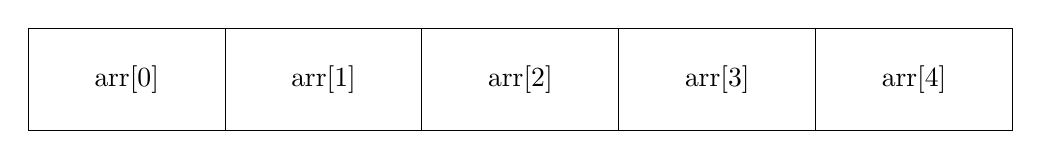
\begin{tikzpicture}[scale=0.5]
		\draw[-] (0,0) -- (5,0) -- (10,0) -- (15,0) -- (20,0) -- (25,0) -- (25,2.6) -- (20,2.6) -- (15,2.6) -- (10,2.6) -- (5,2.6) -- (0,2.6) -- (0,0);
		\draw[-] (5,0) -- (5,2.6);
		\draw[-] (10,0) -- (10,2.6);
		\draw[-] (15,0) -- (15,2.6);
		\draw[-] (20,0) -- (20,2.6);

		\draw (2.5,1.3) node {arr[0]};
		\draw (7.5,1.3) node {arr[1]};
		\draw (12.5,1.3) node {arr[2]};
		\draw (17.5,1.3) node {arr[3]};
		\draw (22.5,1.3) node {arr[4]};
	\end{tikzpicture}
\end{figure}

如果在声明数组时没有指定数组的大小,那么将根据初始化的元素个数来确定。

\vspace{-0.5cm}

\begin{lstlisting}[language=C]
int arr[] = {3, 6, 8, 2, 4, 0, 1, 7};
\end{lstlisting}

通过下标可以访问数组中的元素,下标的有效范围是0 $ \sim $ 数组的长度 - 1,如果使用不合法的下标就会导致数组越界。

\vspace{-0.5cm}

\begin{lstlisting}[language=C]
printf("%d\n", arr[0]);		// 3
printf("%d\n", arr[3]);		// 2
printf("%d\n", arr[7]);		// 7
\end{lstlisting}

当数组的容量比较大时,可以使用循环来初始化数组。

\vspace{-0.5cm}

\begin{lstlisting}[language=C]
int arr[10];

for(int i = 0; i < 10; i++) {
	arr[i] = i + 1;
}
\end{lstlisting}

\vspace{0.5cm}

\mybox{查找数据}

\begin{lstlisting}[language=C]
#include <stdio.h>
#include <stdbool.h>

int main() {
	int n;
	printf("Enter the number of elements: ");
	scanf("%d", &n);

	int arr[n];
	printf("Enter the elements: ");
	for (int i = 0; i < n; i++) {
		scanf("%d", &arr[i]);
	}

	int key;
	printf("Enter the key: ");
	scanf("%d", &key);

	bool found = false;
	for (int i = 0; i < n; i++) {
		if (arr[i] == key) {
			found = true;
			break;
		}
	}

	if (found) {
		printf("%d exists.\n", key);
	} else {
		printf("%d not found!\n", key);
	}

	return 0;
}
\end{lstlisting}

\begin{tcolorbox}
	\mybox{运行结果}
	\begin{verbatim}
Enter the number of elements: 5
Enter the elements: 4 8 9 2 3
Enter the key: 2
2 exists.
	\end{verbatim}
\end{tcolorbox}

\vspace{0.5cm}

\mybox{最大值/最小值}

\begin{lstlisting}[language=C]
#include <stdio.h>

int main() {
	int num[] = {7, 6, 2, 9, 3, 1, 4, 0, 5, 8};
	int n = sizeof(num) / sizeof(num[0]);
	int max = num[0];
	int min = num[0];

	for(int i = 1; i < n; i++) {
		if(num[i] > max) {
			max = num[i];
		}
		if(num[i] < min) {
			min = num[i];
		}
	}

	printf("Max = %d\n", max);
	printf("Min = %d\n", min);
	return 0;
}
\end{lstlisting}

\begin{tcolorbox}
	\mybox{运行结果}
	\begin{verbatim}
Max = 9
Min = 0
	\end{verbatim}
\end{tcolorbox}

\vspace{0.5cm}

\subsection{二维数组(2-Dimensional Array)}

二维数组由行和列两个维度组成,行和列的下标同样也都是从0开始。在声明二维数组时,需要指定行和列的大小。二维数组可以看成是由多个一维数组组成的,因此二维数组中的每个元素都是一个一维数组。

\vspace{-0.5cm}

\begin{lstlisting}[language=C]
int arr[3][4] = {{1, 2, 3, 4}, {5, 6, 7, 8}, {9, 10, 11, 12}};
\end{lstlisting}

\begin{table}[H]
	\centering
	\setlength{\tabcolsep}{5mm}{
		\begin{tabular}{|c|c|c|c|}
			\hline
			arr[0][0] & arr[0][1] & arr[0][2] & arr[0][3] \\
			\hline
			arr[1][0] & arr[1][1] & arr[1][2] & arr[1][3] \\
			\hline
			arr[2][0] & arr[2][1] & arr[2][2] & arr[2][3] \\
			\hline
		\end{tabular}
	}
\end{table}

在初始化二维数组时,为了能够更直观地看出二维数组的结构,可以将每一行单独写在一行中。

\vspace{-0.5cm}

\begin{lstlisting}[language=C]
int arr[3][4] = {
	{1, 2, 3, 4},
	{5, 6, 7, 8},
	{9, 10, 11, 12},
};
\end{lstlisting}

对于容量较大的二维数组,可以通过两层循环进行初始化。

\vspace{-0.5cm}

\begin{lstlisting}[language=C]
int arr[3][4];

for(int i = 0; i < 3; i++) {
	for(int j = 0; j < 4; j++) {
		arr[i][j] = 0;
	}
}
\end{lstlisting}

\vspace{0.5cm}

\mybox{矩阵运算}

\begin{align}\nonumber
	\left[\begin{matrix}
			1 & 3 \\
			1 & 0 \\
			1 & 2 \\
		\end{matrix} \right]
	+
	\left[\begin{matrix}
			0 & 0 \\
			7 & 5 \\
			2 & 1 \\
		\end{matrix} \right]
	=
	\left[\begin{matrix}
			1+0 & 3+0 \\
			1+7 & 0+5 \\
			1+2 & 2+1 \\
		\end{matrix} \right]
	=
	\left[\begin{matrix}
			1 & 3 \\
			8 & 5 \\
			3 & 3 \\
		\end{matrix} \right]
\end{align}

\begin{align}\nonumber
	\left[\begin{matrix}
			1 & 3 \\
			1 & 0 \\
			1 & 2 \\
		\end{matrix} \right]
	-
	\left[\begin{matrix}
			0 & 0 \\
			7 & 5 \\
			2 & 1 \\
		\end{matrix} \right]
	=
	\left[\begin{matrix}
			1-0 & 3-0 \\
			1-7 & 0-5 \\
			1-2 & 2-1 \\
		\end{matrix} \right]
	=
	\left[\begin{matrix}
			1  & 3  \\
			-6 & -5 \\
			-1 & 1  \\
		\end{matrix} \right]
\end{align}

\begin{lstlisting}[language=C]
#include <stdio.h>

int main() {
	int A[3][2] = {
		{1, 3},
		{1, 0},
		{1, 2}
	};
	int B[3][2] = {
		{0, 0},
		{7, 5},
		{2, 1}
	};
	int C[3][2];

	printf("Matrix Addition\n");
	for(int i = 0; i < 3; i++) {
		for(int j = 0; j < 2; j++) {
			C[i][j] = A[i][j] + B[i][j];
			printf("%3d", C[i][j]);
		}
		printf("\n");
	}
	
	printf("Matrix Subtraction\n");
	for(int i = 0; i < 3; i++) {
		for(int j = 0; j < 2; j++) {
			C[i][j] = A[i][j] - B[i][j];
			printf("%3d", C[i][j]);
		}
		printf("\n");
	}
	
	return 0;
}
\end{lstlisting}

\begin{tcolorbox}
	\mybox{运行结果}
	\begin{verbatim}
Matrix Addition
1  3
8  5
3  3
Matrix Subtraction
1  3
-6 -5
-1  1
	\end{verbatim}
\end{tcolorbox}

\newpage

\section{字符串}

\subsection{ASCII}

美国信息交换标准代码ASCII(American Standard Code for Information Interchange)一共定义了128个字符。\\

\begin{longtable}{|c|c|c|c|c|c|c|c|}
	\hline
	\textbf{ASCII} & \textbf{字符} & \textbf{ASCII} & \textbf{字符} & \textbf{ASCII} & \textbf{字符}          & \textbf{ASCII} & \textbf{字符}          \\
	\hline
	0              & NUT           & 32             & (space)       & 64             & @                      & 96             & \lstinline|`| \\
	\hline
	1              & SOH           & 33             & !             & 65             & A                      & 97             & a                      \\
	\hline
	2              & STX           & 34             & \text{"}      & 66             & B                      & 98             & b                      \\
	\hline
	3              & ETX           & 35             & \#            & 67             & C                      & 99             & c                      \\
	\hline
	4              & EOT           & 36             & \$            & 68             & D                      & 100            & d                      \\
	\hline
	5              & ENQ           & 37             & \%            & 69             & E                      & 101            & e                      \\
	\hline
	6              & ACK           & 38             & \&            & 70             & F                      & 102            & f                      \\
	\hline
	7              & BEL           & 39             & \text{'}      & 71             & G                      & 103            & g                      \\
	\hline
	8              & BS            & 40             & (             & 72             & H                      & 104            & h                      \\
	\hline
	9              & HT            & 41             & )             & 73             & I                      & 105            & i                      \\
	\hline
	10             & LF            & 42             & *             & 74             & J                      & 106            & j                      \\
	\hline
	11             & VT            & 43             & +             & 75             & K                      & 107            & k                      \\
	\hline
	12             & FF            & 44             & ,             & 76             & L                      & 108            & l                      \\
	\hline
	13             & CR            & 45             & -             & 77             & M                      & 109            & m                      \\
	\hline
	14             & SO            & 46             & .             & 78             & N                      & 110            & n                      \\
	\hline
	15             & SI            & 47             & /             & 79             & O                      & 111            & o                      \\
	\hline
	16             & DLE           & 48             & 0             & 80             & P                      & 112            & p                      \\
	\hline
	17             & DC1           & 49             & 1             & 81             & Q                      & 113            & q                      \\
	\hline
	18             & DC2           & 50             & 2             & 82             & R                      & 114            & r                      \\
	\hline
	19             & DC3           & 51             & 3             & 83             & S                      & 115            & s                      \\
	\hline
	20             & DC4           & 52             & 4             & 84             & T                      & 116            & t                      \\
	\hline
	21             & NAK           & 53             & 5             & 85             & U                      & 117            & u                      \\
	\hline
	22             & SYN           & 54             & 6             & 86             & V                      & 118            & v                      \\
	\hline
	23             & TB            & 55             & 7             & 87             & W                      & 119            & w                      \\
	\hline
	24             & CAN           & 56             & 8             & 88             & X                      & 120            & x                      \\
	\hline
	25             & EM            & 57             & 9             & 89             & Y                      & 121            & y                      \\
	\hline
	26             & SUB           & 58             & :             & 90             & Z                      & 122            & z                      \\
	\hline
	27             & ESC           & 59             & ;             & 91             & [                      & 123            & \{                     \\
			\hline
	28             & FS            & 60             & <             & 92             & $ \backslash $         & 124            & |                      \\
			\hline
	29             & GS            & 61             & =             & 93             & ]                      & 125            & \}                     \\
	\hline
	30             & RS            & 62             & >             & 94             & \lstinline|^| & 126            & \lstinline|~| \\
	\hline
	31             & US            & 63             & ?             & 95             & \_                     & 127            & DEL                    \\
	\hline
\end{longtable}

\vspace{0.5cm}

\mybox{ASCII}

\begin{lstlisting}[language=C]
#include <stdio.h>

int main() {
	for(int i = 0; i < 128; i++) {
		printf("%d - %c\n", i, i);
	}
	return 0;
}
\end{lstlisting}

\vspace{0.5cm}

\subsection{字符串(String)}

字符数组通常被称为字符串,字符串有两种初始化的方式。一种与普通数组的初始化类似,逐个写出每一个字符,最后需要手动添加$ \backslash $0字符,表示字符串的结束符;另一种是直接使用双引号,这种写法无需手动添加$ \backslash $0。

\vspace{-0.5cm}

\begin{lstlisting}[language=C]
char str[8] = {'p', 'r', 'o', 'g', 'r', 'a', 'm', '\0'};
char str[8] = "program";
\end{lstlisting}

$ \backslash $0占一个字符的大小,因此在设置字符串的大小时需要考虑$ \backslash $0。\\

占位符\%s可以对字符串进行输入输出操作,使用scanf()和gets()都可以用于读取字符串,但是scanf()只会读取到空格为止,而gets()会读取到回车为止。\\

\mybox{字符串输入输出}

\begin{lstlisting}[language=C]
#include <stdio.h>

int main() {
	char str1[32];
	printf("Enter string 1: ");
	gets(str1);
	puts(str1);

	char str2[32];
	printf("Enter string 2: ");
	scanf("%s", str2);
	printf("%s\n", str2);

	return 0;
}
\end{lstlisting}

\begin{tcolorbox}
	\mybox{运行结果}
	\begin{verbatim}
Enter string 1: hello world
hello world
Enter string 2: hello world
hello
	\end{verbatim}
\end{tcolorbox}

\vspace{0.5cm}

\mybox{字符统计}

\begin{lstlisting}[language=C]
#include <stdio.h>

int main() {
	char str[32];
	printf("Enter a string: ");
	gets(str);
	printf("Character to search: ");
	char c = getchar();

	int cnt = 0;
	int i = 0;
	while (str[i] != '\0') {
		if (str[i] == c) {
			cnt++;
		}
		i++;
	}

	printf("\'%c\' appears %d times in \"%s\".\n", c, cnt, str);
	return 0;
}
\end{lstlisting}

\begin{tcolorbox}
	\mybox{运行结果}
	\begin{verbatim}
Enter a string: this is a test
Character to search: t
't' appears 3 times in "this is a test".
	\end{verbatim}
\end{tcolorbox}

\vspace{0.5cm}

\subsection{字符串函数}

头文件<string.h>中定义了一些常用的字符串处理函数。

\subsubsection{strlen()}

计算字符串的长度。\\

\mybox{strlen()}

\begin{lstlisting}[language=C]
#include <stdio.h>
#include <string.h>

int main() {
	char s[] = "hello world";
	printf("Length: %d\n", strlen(s));
	return 0;
}
\end{lstlisting}

\begin{tcolorbox}
	\mybox{运行结果}
	\begin{verbatim}
Length: 11
	\end{verbatim}
\end{tcolorbox}

\vspace{0.5cm}

\subsubsection{strcpy()}

字符串复制,调用者需要确保字符串的大小足够。\\

\mybox{strcpy()}

\begin{lstlisting}[language=C]
#include <stdio.h>
#include <string.h>

int main() {
	char s1[32] = "hello world";
	char s2[32] = "program";

	strcpy(s1, s2);
	printf("s1 = %s\n", s1);
	printf("s2 = %s\n", s2);
	return 0;
}
\end{lstlisting}

\begin{tcolorbox}
	\mybox{运行结果}
	\begin{verbatim}
s1 = program
s2 = program
	\end{verbatim}
\end{tcolorbox}

\vspace{0.5cm}

\subsubsection{strcat()}

字符串拼接,调用者需要确保字符串的大小足够。\\

\mybox{strcat()}

\begin{lstlisting}[language=C]
#include <stdio.h>
#include <string.h>

int main() {
	char s1[32] = "hello";
	char s2[32] = "world";

	strcat(s1, s2);
	printf("s1 = %s\n", s1);
	printf("s2 = %s\n", s2);
	return 0;
}
\end{lstlisting}

\begin{tcolorbox}
	\mybox{运行结果}
	\begin{verbatim}
s1 = helloworld
s2 = world
	\end{verbatim}
\end{tcolorbox}

\vspace{0.5cm}

\subsubsection{strcmp()}

字符串比较,依次比较字符串中每个字符的ASCII码值。通过判断strcmp()的返回值,可以得知两个字符串比较后的结果。

\begin{itemize}
	\item 负数:字符串1 < 字符串2
	\item 正数:字符串1 > 字符串2
	\item 0:字符串1 == 字符串2
\end{itemize}

\vspace{0.5cm}

\mybox{strcmp()}

\begin{lstlisting}[language=C]
#include <stdio.h>
#include <string.h>

int main() {
	char s1[32] = "communication";
	char s2[32] = "compare";
	printf("%d\n", strcmp(s1, s2));
	return 0;
}
\end{lstlisting}

\begin{tcolorbox}
	\mybox{运行结果}
	\begin{verbatim}
-1
	\end{verbatim}
\end{tcolorbox}

\vspace{0.5cm}

\subsection{字符串数组}

字符串数组是一个二维的字符数组,或者可以理解为是由多个字符串组成的数组。

\vspace{-0.5cm}

\begin{lstlisting}[language=C]
char str[4][12] = {"C++", "Java", "Python", "JavaScript"};
\end{lstlisting}

\begin{table}[H]
	\centering
	\setlength{\tabcolsep}{4mm}{
		\begin{tabular}{|c|c|c|c|c|c|c|c|c|c|c|c|c|}
			\hline
			           & \textbf{0} & \textbf{1} & \textbf{2} & \textbf{3}      & \textbf{4}      & \textbf{5} & \textbf{6}      & \textbf{7} & \textbf{8} & \textbf{9} & \textbf{10}     & \textbf{11} \\
			\hline
			\textbf{0} & C          & +          & +          & $ \backslash $0 &                 &            &                 &            &            &            &                 &             \\
			\hline
			\textbf{1} & J          & a          & v          & a               & $ \backslash $0 &            &                 &            &            &            &                 &             \\
			\hline
			\textbf{2} & P          & y          & t          & h               & o               & n          & $ \backslash $0 &            &            &            &                 &             \\
			\hline
			\textbf{3} & J          & a          & v          & a               & S               & c          & r               & i          & p          & t          & $ \backslash $0 &             \\
			\hline
		\end{tabular}
	}
\end{table}

\begin{lstlisting}[language=C]
printf("str[0] = %s\n", str[0]);		// C++
printf("str[1] = %s\n", str[1]);		// Java
printf("str[0][0] = %c\n", str[0][0]);	// C
printf("str[0][1] = %c\n", str[0][1]);	// +
\end{lstlisting}

\newpage
% \chapter{函数}

\section{函数}

\subsection{函数(Function)}

数学中的函数$ y = f(x) $,通过输入$ x $的值,经过计算可以得到$ y $的值。计算机中的函数也是如此,将输入传给函数,经过处理后,会得到输出。\\

函数是一段可重复使用的代码,做了一个特定的任务。例如printf()和strlen()就是函数,其中printf()的功能是输出字符串,strlen()的功能是计算字符串的长度。\\

\begin{figure}[H]
	\centering
	\begin{tikzpicture}[scale=0.5]
		\draw[-] (5,-2) -- (10,-2) -- (10,2) -- (5,2) -- (5,-2);
		\draw[->] (0,0) -- (5,0);
		\draw[->] (10,0) -- (15,0);

		\draw (-2,0) node {Input};
		\draw (17,0) node {Output};
		\draw (7.5,0) node {Function};
	\end{tikzpicture}
	\caption{函数}
\end{figure}

除了这些内置的函数以外,开发者还可以自定义函数,将程序中会被多次使用的代码或做了一件特定的任务的代码写成一个函数,这样就能避免重复写相同的代码,提高开发效率,也利于维护。\\

在编写函数时需要:

\begin{enumerate}
	\item 确定函数的功能
	      \begin{itemize}
		      \item 函数名
		      \item 确保一个函数只做一件事
	      \end{itemize}

	\item 确定函数的输入(参数)
	      \begin{itemize}
		      \item 是否需要参数
		      \item 参数个数
		      \item 参数类型
	      \end{itemize}

	\item 确定函数的输出(返回值)
	      \begin{itemize}
		      \item 是否需要返回值
		      \item 返回值类型
	      \end{itemize}
\end{enumerate}

\vspace{0.5cm}

\mybox{最大值}

\begin{lstlisting}[language=C]
#include <stdio.h>

int max(int num1, int num2);  // function prototype

int main() {
	printf("%d\n", max(4, 12));
	printf("%d\n", max(54, 33));
	printf("%d\n", max(-999, -774));
	return 0;
}

int max(int num1, int num2) {
	// if(num1 > num2) {
	//     return num1;
	// } else {
	//     return num2;
	// }

	return num1 > num2 ? num1 : num2;
}
\end{lstlisting}

\begin{tcolorbox}
	\mybox{运行结果}
	\begin{verbatim}
12
54
-774
	\end{verbatim}
\end{tcolorbox}

函数也可以没有返回值,因为它执行完函数中的代码,并不需要将结果返回给调用者,此时函数的返回值类型为void。\\

\mybox{棋盘}

\begin{lstlisting}[language=C]
#include <stdio.h>

void print_board(int row, int col) {
	for (int i = 0; i < row; i++) {
		for (int j = 0; j < col - 1; j++) {
			printf("   |");
		}
		printf("\n");

		if (i < row - 1) {
			printf("---+---+---\n");
		}
	}
}

int main() {
	print_board(3, 3);
	return 0;
}
\end{lstlisting}

\begin{tcolorbox}
	\mybox{运行结果}
	\begin{verbatim}
   |   |
---+---+---
   |   |
---+---+---
   |   |
	\end{verbatim}
\end{tcolorbox}

\vspace{0.5cm}

\subsection{函数调用}

当调用函数时,程序会记录下当前的执行位置,并跳转到被调用的函数处执行。当被调用的函数执行结束后,程序会回到之前的位置继续执行。\\

\begin{figure}[H]
	\centering
	\begin{tikzpicture}[]
		\draw (0,4.5) node {Caller};
		\draw[->] (0,4) -- (0,0.5);
		\draw[->] (0,-0.5) -- (0,-4);
		\draw (0,0) node {调用foo()};

		\draw (4,4) node {foo()};
		\draw[->] (4,3) -- (4,0.5);
		\draw[->] (4,-0.5) -- (4,-3);
		\draw (4,0) node {调用bar()};

		\draw (8,3) node {bar()};
		\draw[->] (8,2) -- (8,-2);

		\draw[->] (0.5,0.5) -- (3.5,3);
		\draw[->] (3.5,-3) -- (0.5,-0.5);
		\draw[->] (4.5,0.5) -- (7.5,2);
		\draw[->] (7.5,-2) -- (4.5,-0.5);
	\end{tikzpicture}
	\caption{函数调用}
\end{figure}

\vspace{0.5cm}

\mybox{两点间距离}

\begin{lstlisting}[language=C]
#include <stdio.h>
#include <math.h>

double square(double x) {
	return x * x;
}

double distance(double x1, double y1, double x2, double y2) {
	return sqrt(square(x1 - x2) + square(y1 - y2));
}

int main() {
	double x1, y1, x2, y2;
	printf("Enter (x1, y1): ");
	scanf("%lf%lf", &x1, &y1);
	printf("Enter (x2, y2): ");
	scanf("%lf%lf", &x2, &y2);

	printf("Distance: %.2f\n", distance(x1, y1, x2, y2));

	return 0;
}
\end{lstlisting}

\begin{tcolorbox}
	\mybox{运行结果}
	\begin{verbatim}
Enter (x1, y1): 0 0
Enter (x2, y2): 3 4
Distance: 5.00
	\end{verbatim}
\end{tcolorbox}

\newpage

\section{作用域}

\subsection{局部变量(Local Variable)}

定义在块中的变量称为局部变量,在进入块时变量才会被创建,当离开块时变量就会被销毁。因此,局部变量的生存周期为从声明时开始到所在块结束。\\

例如有些变量只在程序的某一段代码中使用,而在其它地方不会被使用。这时就可以将这些变量定义在一个块(if、for、函数等)中,这样可以避免变量名冲突的问题。最典型的一个例子就是在for循环中,循环变量i被定义被块中,因为i的作用仅用于控制循环次数,在离开循环后就没有存在的必要了。

\vspace{-0.5cm}

\begin{lstlisting}[language=C]
for(int i = 0; i < 5; i++)
\end{lstlisting}

块与块之间的变量是互相独立的,即使变量名相同,它们也不是同一个变量。\\

例如在函数调用中,函数的参数也是局部变量,它们的作用域仅限于函数内。\\

例如一个用于交换两个变量的函数swap(),在main()中的变量a和b与swap()中的a和b并不是同一个变量。在调用swap()时,是将main()中的a和b的值复制给swap()中的a和b。swap()交换的是其内部的局部变量,并不会对main()中的a和b产生任何影响。\\

\mybox{局部变量}

\begin{lstlisting}[language=C]
#include <stdio.h>

void swap(int a, int b) {
	int temp = a;
	a = b;
	b = temp;
	printf("swap(): a = %d, b = %d\n", a, b);
}

int main() {
	int a = 1;
	int b = 2;

	printf("Before: a = %d, b = %d\n", a, b);
	swap(a, b);
	printf("After: a = %d, b = %d\n", a, b);

	return 0;
}
\end{lstlisting}

\begin{tcolorbox}
	\mybox{运行结果}
	\begin{verbatim}
Before: a = 1, b = 2
swap(): a = 2, b = 1
After: a = 1, b = 2
	\end{verbatim}
\end{tcolorbox}

\vspace{0.5cm}

\subsection{全局变量(Global Variable)}

全局变量拥有比局部变量更长的生命周期,它的生命周期贯穿整个程序。全局变量可以被程序中所有函数访问。\\

全局变量一般用于:

\begin{itemize}
	\item 定义在整个程序中都会被使用到的常量(例如数组容量)
	\item 被函数间共享的变量(例如计数器)
\end{itemize}

\vspace{0.5cm}

\mybox{全局变量}

\begin{lstlisting}[language=C]
#include <stdio.h>

int a, b;

void swap() {
	int temp = a;
	a = b;
	b = temp;
	printf("swap(): a = %d, b = %d\n", a, b);
}

int main() {
	a = 1;
	b = 2;

	printf("Before: a = %d, b = %d\n", a, b);
	swap(a, b);
	printf("After: a = %d, b = %d\n", a, b);

	return 0;
}
\end{lstlisting}

\begin{tcolorbox}
	\mybox{运行结果}
	\begin{verbatim}
Before: a = 1, b = 2
swap(): a = 2, b = 1
After: a = 2, b = 1
	\end{verbatim}
\end{tcolorbox}

\newpage

\section{递归} \label{recursion}

\subsection{递归(Recursion)}

要理解递归,得先理解递归(见\ref{recursion}章节)。\\

一个函数调用自己的过程被称为递归。递归可以轻松地解决一些复杂的问题,很多著名的算法都利用了递归的思想。

\begin{figure}[H]
	\centering
	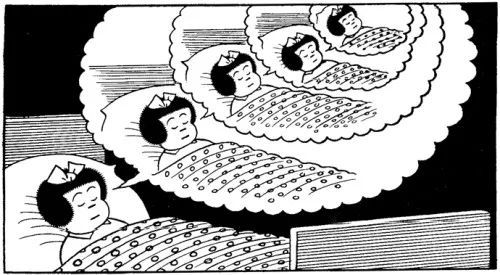
\includegraphics[scale=0.7]{img/Chapter5/5-3/1.png}
\end{figure}

\vspace{0.5cm}

\mybox{讲故事}

\begin{lstlisting}[language=C]
#include <stdio.h>
#include <string.h>

void tell_story() {
	char story[1024] = {0};
	strcat(story, "从前有座山,山里有座庙\n");
	strcat(story, "庙里有个老和尚\n");
	strcat(story, "老和尚在对小和尚讲故事:\n");
	printf("%s", story);

	tell_story();
}

int main() {
	tell_story();
	return 0;
}
\end{lstlisting}

\begin{tcolorbox}
	\mybox{运行结果}
	\begin{verbatim}
从前有座山,山里有座庙
庙里有个老和尚
老和尚在对小和尚讲故事:
从前有座山,山里有座庙
庙里有个老和尚
老和尚在对小和尚讲故事:
从前有座山,山里有座庙
庙里有个老和尚
老和尚在对小和尚讲故事:
...
	\end{verbatim}
\end{tcolorbox}

一个永远无法结束的递归函数最终会导致栈溢出。因此递归函数需要确定一个结束条件,确保在递归过程中能在合适的地方停止并返回。\\

\mybox{阶乘}

\begin{lstlisting}[language=C]
#include <stdio.h>

int factorial(int n) {
    if(n == 0 || n == 1) {
        return 1;
    }
    return n * factorial(n-1);
}

int main() {
    printf("5! = %d\n", factorial(5));
    return 0;
}
\end{lstlisting}

\begin{tcolorbox}
	\mybox{运行结果}
	\begin{verbatim}
5! = 120
	\end{verbatim}
\end{tcolorbox}

\begin{figure}[H]
	\centering
	\begin{tikzpicture}[]
		\draw (0,0) rectangle (3,1.5);
		\draw (3,-2) rectangle (6,-0.5);
		\draw (6,-4) rectangle (9,-2.5);
		\draw (9,-6) rectangle (12,-4.5);
		\draw (12,-8) rectangle (15,-6.5);

		\draw (12.75,-10.75) rectangle (14.25,-9.25);
		\draw (9.75,-8.75) rectangle (11.25,-7.25);
		\draw (6.75,-6.75) rectangle (8.25,-5.25);
		\draw (3.75,-4.75) rectangle (5.25,-3.25);
		\draw (0.75,-2.75) rectangle (2.25,-1.25);

		\draw (1.5,0.75) node {$ factorial(5) $};
		\draw (4.5,-1.25) node {$ factorial(4) $};
		\draw (7.5,-3.25) node {$ factorial(3) $};
		\draw (10.5,-5.25) node {$ factorial(2) $};
		\draw (13.5,-7.25) node {$ factorial(1) $};

		\draw (13.5,-10) node {$ 1 $};
		\draw (10.5,-8) node {$ 2 $};
		\draw (7.5,-6) node {$ 6 $};
		\draw (4.5,-4) node {$ 24 $};
		\draw (1.5,-2) node {$ 120 $};

		\draw[->] (3,0.75) -- (4.5,0.75) -- (4.5,-0.5);
		\draw[->] (6,-1.25) -- (7.5,-1.25) -- (7.5,-2.5);
		\draw[->] (9,-3.25) -- (10.5,-3.25) -- (10.5,-4.5);
		\draw[->] (12,-5.25) -- (13.5,-5.25) -- (13.5,-6.5);

		\draw[->] (12.75,-10) -- (10.5,-10) -- (10.5,-8.75);
		\draw[->] (9.75,-8) -- (7.5,-8) -- (7.5,-6.75);
		\draw[->] (6.75,-6) -- (4.5,-6) -- (4.5,-4.75);
		\draw[->] (3.75,-4) -- (1.5,-4) -- (1.5,-2.75);

		\draw (4.5,1) node {$ 5 * factorial(4) $};
		\draw (7.5,-1) node {$ 4 * factorial(3) $};
		\draw (10.5,-3) node {$ 3 * factorial(2) $};
		\draw (13.5,-5) node {$ 2 * factorial(1) $};

		\draw (11,-10.5) node {$ 2 * 1 $};
		\draw (8,-8.5) node {$ 3 * 2 $};
		\draw (5,-6.5) node {$ 4 * 6 $};
		\draw (2,-4.5) node {$ 5 * 24 $};
	\end{tikzpicture}
	\caption{阶乘}
\end{figure}

\vspace{0.5cm}

\mybox{斐波那契数列}

\begin{lstlisting}[language=C]
#include <stdio.h>

int fibonacci(int n) {
	if (n == 1 || n == 2) {
		return 1;
	}
	return fibonacci(n - 2) + fibonacci(n - 1);
}

int main() {
	int n = 7;
	printf("%d\n", fibonacci(n));
	return 0;
}
\end{lstlisting}

\begin{tcolorbox}
	\mybox{运行结果}
	\begin{verbatim}
13
	\end{verbatim}
\end{tcolorbox}

\begin{figure}[H]
	\centering
	\begin{tikzpicture}[
			level distance=2.4cm,
			level 1/.style={sibling distance=6cm},
			level 2/.style={sibling distance=3cm},
			level 3/.style={sibling distance=2cm}
		]
		\node {$ f(5) $}
		child {
				node {$ f(3) $}
				child {node {$ f(1) $}}
				child {node {$ f(2) $}}
			}
		child {
				node {$ f(4) $}
				child {node {$ f(2) $}}
				child {
						node {$ f(3) $}
						child {node {$ f(1) $}}
						child {node {$ f(2) $}}
					}
			};
	\end{tikzpicture}
	\caption{递归树}
\end{figure}

递归的特点就是将一个复杂的大问题逐步简化为一个可以解决的小问题,然后再逐步计算出大问题的解。\\

递归的优点在于代码简洁易懂,但是缺点也很明显,就是效率很低。每次递归都会产生函数调用,而函数调用的开销是很大的,不适合用来解决大规模的问题。\\

例如在计算斐波那契数列的第40项时,递归需要花费大量时间,因为其中包含了大量的重复计算。相比而言,使用循环的方式能够节省大量的时间。因此像阶乘和斐波那契数列这样的情况,通常会采用循环,而不是递归进行计算。\\

然而还存在很多问题不得不使用递归的思想才能解决。\\

\mybox{阿克曼函数}

\begin{align}\nonumber
	A(m, n) =
	\begin{cases}
		n + 1             & m = 0        \\
		A(m-1, 1)         & m > 0, n = 0 \\
		A(m-1, A(m, n-1)) & m > 0, n > 0 \\
	\end{cases}
\end{align}

\begin{lstlisting}[language=C]
#include <stdio.h>

int A(int m, int n) {
	if (m == 0) {
		return n + 1;
	} else if (m > 0 && n == 0) {
		return A(m - 1, 1);
	} else {
		return A(m - 1, A(m, n - 1));
	}
}

int main() {
	printf("%d\n", A(3, 4));
	return 0;
}
\end{lstlisting}

\begin{tcolorbox}
	\mybox{运行结果}
	\begin{verbatim}
125
	\end{verbatim}
\end{tcolorbox}

\vspace{0.5cm}

\mybox{汉诺塔}\\

给定三根柱子,其中A柱子从大到小套有n个圆盘,问题是如何借助B柱子,将圆盘从A搬到C。\\

规则:

\begin{itemize}
	\item 一次只能搬动一个圆盘
	\item 不能将大圆盘放在小圆盘上面
\end{itemize}

\begin{figure}[H]
	\centering
	
\includegraphics[scale=0.4]{img/Chapter5/5-3/3.png}
\end{figure}

递归算法求解汉诺塔问题:

\begin{enumerate}
	\item 将前n-1个圆盘从A柱借助于C柱搬到B柱。
	\item 将最后一个圆盘直接从A柱搬到C柱。
	\item 将n-1个圆盘从B柱借助于A柱搬到C柱。
\end{enumerate}

\begin{lstlisting}[language=C]
#include <stdio.h>

int move = 0;

void hanoi(int n, char src, char mid, char dst) {
	if (n == 1) {
		printf("%c -> %c\n", src, dst);
		move++;
	} else {
		// move top n-1 disks from src to mid
		hanoi(n - 1, src, dst, mid);
		printf("%c -> %c\n", src, dst);
		move++;
		// move top n-1 disks from mid to dst
		hanoi(n - 1, mid, src, dst);
	}
}

int main() {
	hanoi(4, 'A', 'B', 'C');
	printf("Moves: %d\n", move);
	return 0;
}
\end{lstlisting}

\begin{tcolorbox}
	\mybox{运行结果}
	\begin{verbatim}
A -> B
A -> C
B -> C
A -> B
C -> A
C -> B
A -> B
A -> C
B -> C
B -> A
C -> A
B -> C
A -> B
A -> C
B -> C
Moves: 15
	\end{verbatim}
\end{tcolorbox}

\begin{figure}[H]
	\centering
	
\includegraphics[]{img/Chapter5/5-3/2.png}
\end{figure}

\newpage
\chapter{函数}

\section{函数}

\subsection{函数(Function)}

函数执行一个特定的任务,C提供了大量内置函数,例如println用来输出字符串、substring()用来截取子字符串等。

\begin{figure}[H]
	\centering
	\begin{tikzpicture}[scale=0.5]
		\draw[-] (5,-2) -- (10,-2) -- (10,2) -- (5,2) -- (5,-2);
		\draw[->] (0,0) -- (5,0);
		\draw[->] (10,0) -- (15,0);

		\draw (-2,0) node {Input};
		\draw (17,0) node {Output};
		\draw (7.5,0) node {Function};
	\end{tikzpicture}
	\caption{函数}
\end{figure}

当调用函数时,程序控制权会转移给被调用的函数,当函数执行结束后,函数会把程序序控制权交还给其调用者。

\begin{figure}[H]
	\centering
	\begin{tikzpicture}[]
		\draw (0,4.5) node {Caller};
		\draw[->] (0,4) -- (0,0.5);
		\draw[->] (0,-0.5) -- (0,-4);
		\draw (0,0) node {调用foo()};

		\draw (4,4) node {foo()};
		\draw[->] (4,3) -- (4,0.5);
		\draw[->] (4,-0.5) -- (4,-3);
		\draw (4,0) node {调用bar()};

		\draw (8,3) node {bar()};
		\draw[->] (8,2) -- (8,-2);

		\draw[->] (0.5,0.5) -- (3.5,3);
		\draw[->] (3.5,-3) -- (0.5,-0.5);
		\draw[->] (4.5,0.5) -- (7.5,2);
		\draw[->] (7.5,-2) -- (4.5,-0.5);
	\end{tikzpicture}
	\caption{函数调用}
\end{figure}

函数声明时需要指定函数的名称、返回类型和参数。在函数声明时,参数的名称可以省略,但是参数的类型是必须的。\\

函数的参数列表包括参数的类型、顺序、数量等信息,参数列表可以为空。\\

函数可以返回一个值,函数的返回类型为被返回的值的类型。函数也可以不返回任何值,此时函数的返回类型应定义为void。

\begin{lstlisting}[language=C]
AccessModifier dataType funcName(parameterList) {
	//code
}
\end{lstlisting}

\vspace{0.5cm}

\subsection{函数设计方法}

为什么不把所有的代码全部写在一起,还需要自定义函数呢?\\

使用函数有以下好处:

\begin{enumerate}
	\item 避免代码复制,代码复制是程序质量不良的表现
	\item 便于代码维护
	\item 避免重复造轮子,提高开发效率
\end{enumerate}

在设计函数的时候需要考虑以下的几点要素:

\begin{enumerate}
	\item 确定函数的功能

	\item 确定函数的参数
	      \begin{itemize}
		      \item 是否需要参数
		      \item 参数个数
		      \item 参数类型
	      \end{itemize}

	\item 确定函数的返回值
	      \begin{itemize}
		      \item 是否需要返回值
		      \item 返回值类型
	      \end{itemize}
\end{enumerate}

\mybox{函数实现返回最大值}

\begin{lstlisting}[language=C]
public class Max {
	public static void main(String[] args) {
		System.out.println(max(4, 12));
		System.out.println(max(54, 33));
		System.out.println(max(0, -12));
		System.out.println(max(-999, -774));
	}

	public static int max(int num1, int num2) {
		// if(num1 > num2) {
		//	 return num1;
		// } else {
		//	 return num2;
		// }
		return num1 > num2 ? num1 : num2;
	}
}
\end{lstlisting}

\begin{tcolorbox}
	\mybox{运行结果}
	\begin{verbatim}
12
54
0
-774
	\end{verbatim}
\end{tcolorbox}

\vspace{0.5cm}

\mybox{函数实现累加和}

\begin{lstlisting}[language=C]
public class Sum {
	public static void main(String[] args) {
		System.out.println("1-100的累加和 = " + sum(1, 100));
		System.out.println("1024-2048的累加和 = "+ sum(1024, 2048));
	}

	public static int sum(int start, int end) {
		int total = 0;
		for(int i = start; i <= end; i++) {
			total += i;
		}
		return total;
	}
}
\end{lstlisting}

\begin{tcolorbox}
	\mybox{运行结果}
	\begin{verbatim}
1-100的累加和 = 5050
1024-2048的累加和 = 1574400
	\end{verbatim}
\end{tcolorbox}

\vspace{0.5cm}

\mybox{函数实现输出i行j列由自定义字符组成的图案}

\begin{lstlisting}[language=C]
public class PrintChars {
	public static void main(String[] args) {
		printChars(5, 10, '?');
	}

	public static void printChars(int row, int col, char c) {
		for(int i = 0; i < row; i++) {
			for(int j = 0; j < col; j++) {
				System.out.print(c);
			}
			System.out.println();
		}
	}
}
\end{lstlisting}

\begin{tcolorbox}
	\mybox{运行结果}
	\begin{verbatim}
??????????
??????????
??????????
??????????
??????????
	\end{verbatim}
\end{tcolorbox}

\newpage

\section{递归} \label{recursive}

\subsection{递归(Recursion)}

要理解递归,先得理解递归(见\ref{recursive}章节)。\\

在函数的内部,直接或者间接的调用自己的过程就叫作递归。对于一些问题,使用递归可以简洁易懂的解决问题,但是递归的缺点是性能低,占用大量系统栈空间。\\

递归算法很多时候可以处理一些特别复杂、难以直接解决的问题。例如:

\begin{itemize}
	\item 迷宫
	\item 汉诺塔
	\item 八皇后
	\item 排序
	\item 搜索
\end{itemize}

在定义递归函数时,一定要确定一个结束条件,否则会造成无限递归的情况,最终会导致栈溢出。

\begin{figure}[H]
	\centering
	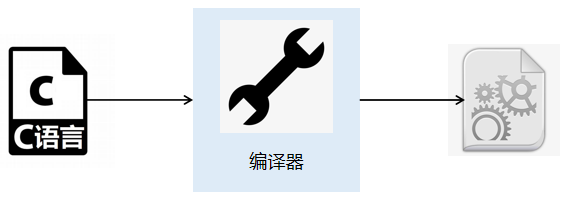
\includegraphics[scale=0.7]{img/C6/6-2/1.png}
\end{figure}

\begin{figure}[H]
	\centering
	
\includegraphics[scale=0.6]{img/C6/6-2/2.png}
\end{figure}

\begin{figure}[H]
	\centering
	
\includegraphics[scale=0.6]{img/C6/6-2/3.png}
\end{figure}

\begin{figure}[H]
	\centering
	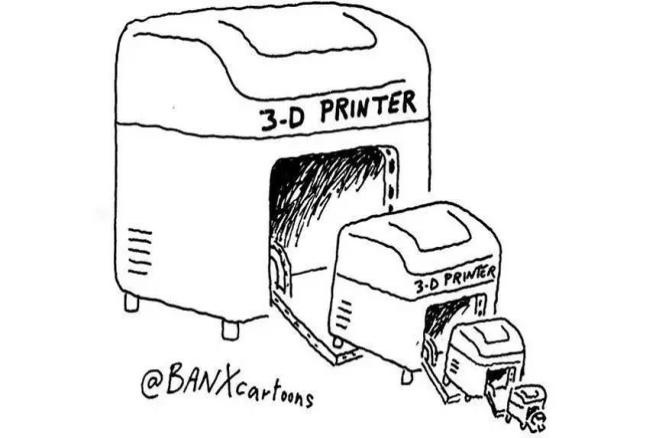
\includegraphics[scale=1.3]{img/C6/6-2/4.png}
\end{figure}

\begin{figure}[H]
	\centering
	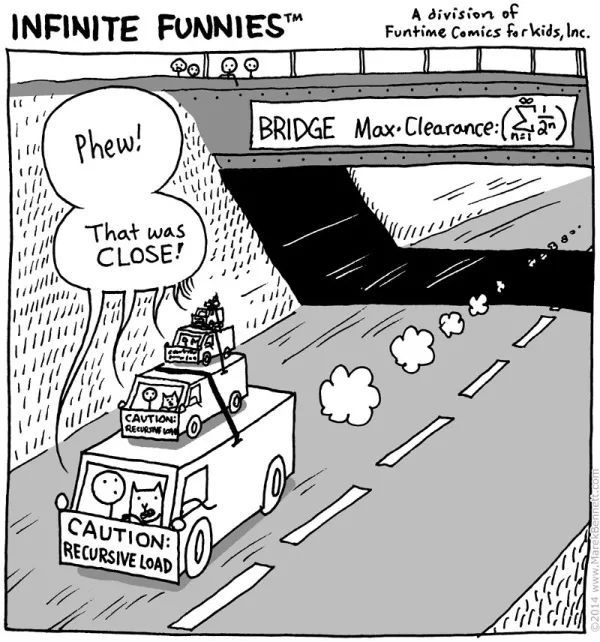
\includegraphics[scale=0.6]{img/C6/6-2/5.png}
\end{figure}

\mybox{无限递归}

\begin{lstlisting}[language=C]
public class TellStory {
	public static void main(String[] args) {
		tellStory();
	}
	
	public static void tellStory() {
		System.out.println("从前有座山");
		System.out.println("山里有座庙");
		System.out.println("庙里有个老和尚和小和尚");
		System.out.println("老和尚在对小和尚讲故");
		System.out.println("他讲的故事是:");
		tellStory();
	}
}
\end{lstlisting}

\begin{tcolorbox}
	\mybox{运行结果}
	\begin{verbatim}
从前有座山
山里有座庙
庙里有个老和尚和小和尚
老和尚对小和尚在讲故事
他讲的故事是:
从前有座山
山里有座庙
庙里有个老和尚和小和尚
老和尚对小和尚在讲故事
他讲的故事是:
...
	\end{verbatim}
\end{tcolorbox}

递归函数一般需要定义递归的出口,即结束条件,确保递归能够在适合的地方退出。\\

\mybox{阶乘}

\begin{lstlisting}[language=C]
public class Factorial {
	public static void main(String[] args) {
		System.out.println("5! = " + factorial(5));
	}
	
	public static int factorial(int n) {
		if(n == 0 || n == 1) {
			return 1;
		}
		return n * factorial(n-1);
	}
}
\end{lstlisting}

\begin{tcolorbox}
	\mybox{运行结果}
	\begin{verbatim}
5! = 120
	\end{verbatim}
\end{tcolorbox}

\begin{figure}[H]
	\centering
	\begin{tikzpicture}[]
		\draw (0,0) rectangle (3,1.5);
		\draw (3,-2) rectangle (6,-0.5);
		\draw (6,-4) rectangle (9,-2.5);
		\draw (9,-6) rectangle (12,-4.5);
		\draw (12,-8) rectangle (15,-6.5);

		\draw (12.75,-10.75) rectangle (14.25,-9.25);
		\draw (9.75,-8.75) rectangle (11.25,-7.25);
		\draw (6.75,-6.75) rectangle (8.25,-5.25);
		\draw (3.75,-4.75) rectangle (5.25,-3.25);
		\draw (0.75,-2.75) rectangle (2.25,-1.25);

		\draw (1.5,0.75) node {$ factorial(5) $};
		\draw (4.5,-1.25) node {$ factorial(4) $};
		\draw (7.5,-3.25) node {$ factorial(3) $};
		\draw (10.5,-5.25) node {$ factorial(2) $};
		\draw (13.5,-7.25) node {$ factorial(1) $};

		\draw (13.5,-10) node {$ 1 $};
		\draw (10.5,-8) node {$ 2 $};
		\draw (7.5,-6) node {$ 6 $};
		\draw (4.5,-4) node {$ 24 $};
		\draw (1.5,-2) node {$ 120 $};

		\draw[->] (3,0.75) -- (4.5,0.75) -- (4.5,-0.5);
		\draw[->] (6,-1.25) -- (7.5,-1.25) -- (7.5,-2.5);
		\draw[->] (9,-3.25) -- (10.5,-3.25) -- (10.5,-4.5);
		\draw[->] (12,-5.25) -- (13.5,-5.25) -- (13.5,-6.5);

		\draw[->] (12.75,-10) -- (10.5,-10) -- (10.5,-8.75);
		\draw[->] (9.75,-8) -- (7.5,-8) -- (7.5,-6.75);
		\draw[->] (6.75,-6) -- (4.5,-6) -- (4.5,-4.75);
		\draw[->] (3.75,-4) -- (1.5,-4) -- (1.5,-2.75);

		\draw (4.5,1) node {$ 5 * factorial(4) $};
		\draw (7.5,-1) node {$ 4 * factorial(3) $};
		\draw (10.5,-3) node {$ 3 * factorial(2) $};
		\draw (13.5,-5) node {$ 2 * factorial(1) $};

		\draw (11,-10.5) node {$ 2 * 1 $};
		\draw (8,-8.5) node {$ 3 * 2 $};
		\draw (5,-6.5) node {$ 4 * 6 $};
		\draw (2,-4.5) node {$ 5 * 24 $};
	\end{tikzpicture}
	\caption{阶乘}
\end{figure}

\mybox{斐波那契数列(递归)}

\begin{lstlisting}[language=C]
public class FibonacciRecursive {
	public static void main(String[] args) {
		int n = 7;
		System.out.println(
			"斐波那契数列第" + n + "位:"+ fibonacci(n)
		);
	}
	
	public static int fibonacci(int n) {
		if(n == 1 || n == 2) {
			return 1;
		}
		return fibonacci(n-2) + fibonacci(n-1);
	}
}
\end{lstlisting}

\begin{tcolorbox}
	\mybox{运行结果}
	\begin{verbatim}
斐波那契数列第7位:13
	\end{verbatim}
\end{tcolorbox}

\begin{figure}[H]
	\centering
	\begin{tikzpicture}[
			level distance=2.4cm,
			level 1/.style={sibling distance=6cm},
			level 2/.style={sibling distance=3cm},
			level 3/.style={sibling distance=2cm}
		]
		\node {$ f(5) $}
		child {
				node {$ f(3) $}
				child {node {$ f(1) $}}
				child {
						node {$ f(2) $}
						child {node {$ f(0) $}}
						child {node {$ f(1) $}}
					}
			}
		child {
				node {$ f(4) $}
				child {
						node {$ f(2) $}
						child {node {$ f(0) $}}
						child {node {$ f(1) $}}
					}
				child {
						node {$ f(3) $}
						child {node {$ f(1) $}}
						child {
								node {$ f(2) $}
								child {node {$ f(0) $}}
								child {node {$ f(1) $}}
							}
					}
			};
	\end{tikzpicture}
	\caption{递归树}
\end{figure}

\mybox{斐波那契数列(迭代)}

\begin{lstlisting}[language=C]
public class FibonacciIterative {
	public static void main(String[] args) {
		int n = 7;
		System.out.println(
			"斐波那契数列第" + n + "位:"+ fibonacci(n)
		);
	}
	
	public static int fibonacci(int n) {
		int[] f = new int[n];
		f[0] = f[1] = 1;
		for(int i = 2; i < n; i++) {
			f[i] = f[i-2] + f[i-1];
		}
		return f[n-1];
	}
}
\end{lstlisting}

\begin{tcolorbox}
	\mybox{运行结果}
	\begin{verbatim}
斐波那契数列第7位:13
	\end{verbatim}
\end{tcolorbox}

\vspace{0.5cm}

\mybox{阿克曼函数}

\begin{align}\nonumber
	A(m, n) =
	\begin{cases}
		n + 1             & m = 0        \\
		A(m-1, 1)         & m > 0, n = 0 \\
		A(m-1, A(m, n-1)) & m > 0, n > 0 \\
	\end{cases}
\end{align}

\begin{lstlisting}[language=C]
public class Ackermann {
	public static void main(String[] args) {
		System.out.println(A(3, 4));
	}
	
	public static int A(int m, int n) {
		if(m == 0) {
			return n + 1;
		} else if(m > 0 && n == 0) {
			return A(m-1, 1);
		} else {
			return A(m-1, A(m, n-1));
		}
	}
}
\end{lstlisting}

\begin{tcolorbox}
	\mybox{运行结果}
	\begin{verbatim}
125
	\end{verbatim}
\end{tcolorbox}

\begin{table}[H]
	\centering
	\setlength{\tabcolsep}{0.5mm}{
		\begin{tabular}{|c|c|c|c|c|c|c|}
			\hline
			\diagbox{$ m $}{$ n $} & \textbf{$ 0 $} & \textbf{$ 1 $}    & \textbf{$ 2 $}    & \textbf{$ 3 $}          & \textbf{$ 4 $}    & \textbf{$ n $}                                         \\
			\hline
			\textbf{$ 0 $}         & $ 1 $          & $ 2 $             & $ 3 $             & $ 4 $                   & $ 5 $             & $ n + 1 $                                              \\
			\hline
			\textbf{$ 1 $}         & $ 2 $          & $ 3 $             & $ 4 $             & $ 5 $                   & $ 6 $             & $ 2 + (n + 3) - 3 $                                    \\
			\hline
			\textbf{$ 2 $}         & $ 3 $          & $ 5 $             & $ 7 $             & $ 9 $                   & $ 11 $            & $ 2(n + 3) - 3 $                                       \\
			\hline
			\textbf{$ 3 $}         & $ 5 $          & $ 13 $            & $ 29 $            & $ 61 $                  & $ 125 $           & $ 2^{n + 3} - 3 $                                      \\
			\hline
			\textbf{$ 4 $}         & $ 13 $         & $ 65533 $         & $ 2^{65536} - 3 $ & $ A(3, 2^{65536} - 3) $ & $ A(3, A(4, 3)) $ & $ \underbrace{2^{2^{.^{.^{.{^2}}}}}}_{n+3\ twos} - 3 $ \\
			\hline
			\textbf{$ 5 $}         & $ 65533 $      & $ A(4, 65533) $   & $ A(4, A(5, 1)) $ & $ A(4, A(5, 2)) $       & $ A(4, A(5, 3)) $ & $ \dots $                                              \\
			\hline
			\textbf{$ 6 $}         & $ A(5, 1) $    & $ A(5, A(5, 1)) $ & $ A(5, A(6, 1)) $ & $ A(5, A(6, 2)) $       & $ A(5, A(6, 3)) $ & $ \dots $                                              \\
			\hline
		\end{tabular}
	}
	\caption{阿克曼函数}
\end{table}

\begin{figure}[H]
	\centering
	
\includegraphics[]{img/C6/6-2/6.png}
\end{figure}

\mybox{汉诺塔}\\

给定三根柱子,其中A柱子从大到小套有n个圆盘,问题是如何借助B柱子,将圆盘从A搬到C。\\

规则:

\begin{itemize}
	\item 一次只能搬动一个圆盘
	\item 不能将大圆盘放在小圆盘上面
\end{itemize}

\begin{figure}[H]
	\centering
	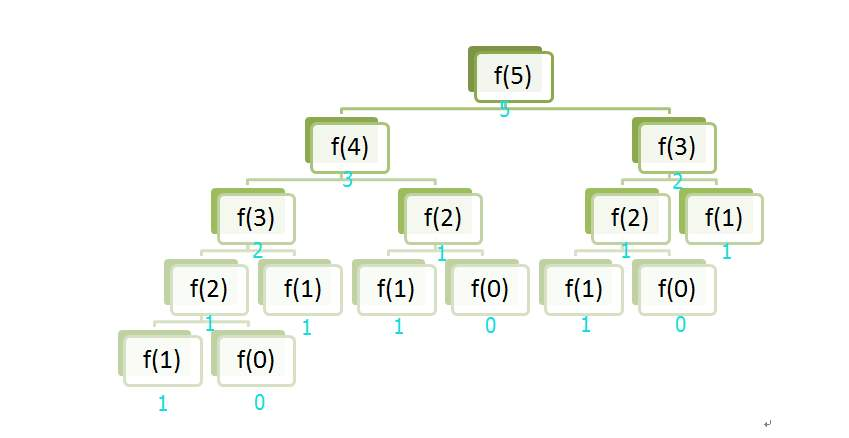
\includegraphics[scale=0.4]{img/C6/6-2/7.png}
\end{figure}

递归算法求解汉诺塔问题:

\begin{enumerate}
	\item 将前n-1个圆盘从A柱借助于C柱搬到B柱。
	\item 将最后一个圆盘直接从A柱搬到C柱。
	\item 将n-1个圆盘从B柱借助于A柱搬到C柱。
\end{enumerate}

\begin{lstlisting}[language=C]
public class Hanoi {
	public static int move = 0;		 // 移动次数
	
	public static void main(String[] args) {
		hanoi(4, 'A', 'B', 'C');
		System.out.println("步数==>" + move);
	}
	
	/**
	 * @brief  汉诺塔算法
	 * @note   把 n 个盘子从 src 借助 mid 移到 dst
	 * @param  n: 层数
	 * @param  src: 起点柱子
	 * @param  mid: 临时柱子
	 * @param  dst: 目标柱子
	 */
	public static void hanoi(int n, char src, char mid, char dst) {
		if(n == 1) {
			System.out.println(n + "号盘:" + src + "->" + dst);
			move++;
		} else {
			// 把前 n-1 个盘子从 src 借助 dst 移到 mid
			hanoi(n-1, src, dst, mid);
			// 移动第 n 个盘子
			System.out.println(n + "号盘:" + src + "->" + dst);
			move++;
			// 把刚才的 n-1 个盘子从 mid 借助 src 移到 dst
			hanoi(n-1, mid, src, dst);
		}
	}
}
\end{lstlisting}

\begin{tcolorbox}
	\mybox{运行结果}
	\begin{verbatim}
1号盘:A -> B
2号盘:A -> C
1号盘:B -> C
3号盘:A -> B
1号盘:C -> A
2号盘:C -> B
1号盘:A -> B
4号盘:A -> C
1号盘:B -> C
2号盘:B -> A
1号盘:C -> A
3号盘:B -> C
1号盘:A -> B
2号盘:A -> C
1号盘:B -> C
步数 ==> 15
	\end{verbatim}
\end{tcolorbox}

\newpage

\end{document}